\documentclass[../../main.tex]{subfiles}

\begin{document}

	\subsection{Reliability}

	The system implementing functionalities needed to access the stores is of greatest importance, thus its 
	infrastructure should be characterized by the highest MTTF and lowest MTTR possible.

	On the other side, all the "remote" functionalities, such as booking via IT device or telephone and notifications, 
	are required to have good reliability, but can afford a slightly higher MTTR than the other system mentioned above. 
	However, it is mandatory to ensure the lack of data losses during downtime.

	\subsection{Availability}

	All services are needed 24/7, so it is needed at least 99.99\% availability (1 minute of down-time per week). 
	Both supermarkets and users need to be notified in case of any communication issues with CLup servers.

	Stores should be able to communicate with CLup's servers during all their opening time span.

	As shown in the following histogram, it is expected an high utilisation of all services during the day, 
	and a low usage during night hours. This means that it is better to do all maintenance activities in the evening, 
	during the night or in the early morning, in order to keep the availability of critical functionalities to its maximum, 
	especially during busy hours.

	\begin{figure}[H]
	    \centering
	    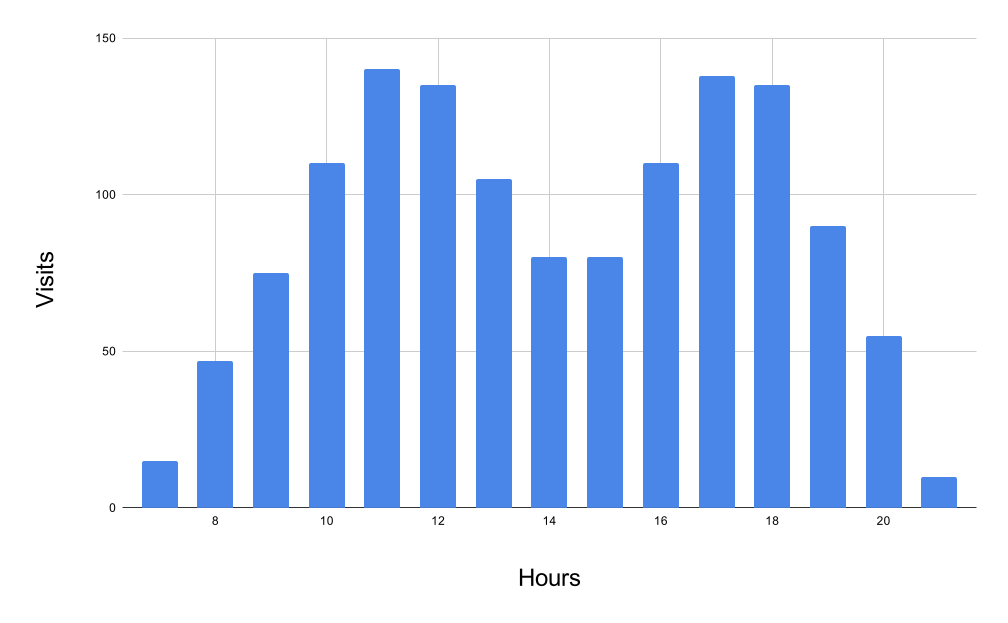
\includegraphics[width=0.8\textwidth]{affluence-chart.png}
	    \caption{Average daily visits in the supermarket in Milan with the most affluence. \\Credits: Google Popular Times (11/2020).}
  	\end{figure}

	\subsection{Security}

	All data inbound to CLup services must be treated as stated by GDPR regulations. 

	Store personnel (i.e., store managers and store assistants) will authenticate to the system using Single Sign On (SSO) integrations with the stores identity systems, using either OAuth or SAML. This will allow the system to delegate the user management to external identity systems, with the benefits of:
	\begin{itemize}
		\item not having to deal with sensitive information (e.g., passwords) \\
		\item inheriting the change of permissions of the users (e.g., a promotion from store assistant to store manager) \\
		\item providing the users with a unified and smooth log in experience (since they will use the same credentials they use to access all other stores' systems)
	\end{itemize}

	Additionally, to guarantee the protection of the customer's data in between servers and the 
	user's device, all Internet traffic must be encrypted with a modern version of TLS, and sent via HTTPS protocol.

	Finally, to guarantee data protection in the backend side, data at rest encryption needs to be used: this way the system should be protected 
	from data breaches and thefts.

	\subsection{Maintainability}

	The back-end system must be designed for sustaining maintenance operations without having to 
	shut down services, guaranteeing no down-time during these operations. For this reason, a dedicated staging environment must be put in place and used to test every new release of the software. The staging environment must be as similar as possible to the production environment, the only difference being the data that it works on: properly anonymized production data.

	All devices inside the supermarkets, like ticket scanners and printers, must support OTA firmware updates. When necessary, these devices will have to be updated when the store is closed, to guarantee the maximum availability.

	Customer's software on smartphones can be updated at any time, through the appropriate app stores.

	\subsection{Portability}

	CLup smartphone application must be available for Android and iOS operating systems. As per compatibility, the Android app must be supported by at least Android KitKat 4.4, while the iOS app must be compatible with at least iOS 12.4.

	All customer side functions must also be provided on the Web platform, in order to be able to access 
	CLup's services by Internet browsers, both from PC and smartphones.

	The software for store managers and employees must be hosted on Web platform, with support for both PC and smartphone layouts.

	
\end{document}
